\documentclass{beamer}
\usefonttheme[onlymath]{serif}
\usepackage[T1]{fontenc}
\usepackage[utf8]{inputenc}
\usepackage[english]{babel}
\usepackage{amsmath}
\usepackage{amssymb}
\usepackage{amsthm}
\usepackage{gensymb}
\usepackage{parskip}
\usepackage{mathtools}
\usepackage{listings}
\usepackage{hyperref}
\usepackage{graphicx}
\usepackage{color}
\usepackage{enumerate}
\usepackage{tikz}
\usetikzlibrary{calc}
\usetikzlibrary{positioning}
\usetikzlibrary{angles}
\usetikzlibrary{shapes}
\usetikzlibrary{arrows}
\usepackage{verbatim}
\usepackage{multicol}
\usepackage{array}
\usepackage{minted}
\parskip 0pt


\DeclareMathOperator{\lcm}{lcm}
\newcommand\floor[1]{\left\lfloor#1\right\rfloor}
\newcommand\ceil[1]{\left\lceil#1\right\rceil}
\newcommand\abs[1]{\left|#1\right|}
\newcommand\p[1]{\left(#1\right)}
\newcommand\sqp[1]{\left[#1\right]}
\newcommand\cp[1]{\left\{#1\right\}}
\newcommand\norm[1]{\left\lVert#1\right\rVert}
\renewcommand\Im{\operatorname{Im}}
\renewcommand\Re{\operatorname{Re}}

\usetheme{metropolis}
\definecolor{dark yellow}{rgb} {0.6,0.6,0.0}
\definecolor{dark green}{rgb} {0.0,0.6,0.0}

\graphicspath{{myndir/}}

\title{Divide and conquer, Dynamic programming}
\author{Arnar Bjarni Arnarson \& Atli FF}
\institute{\href{http://ru.is/td}{School of Computer Science} \\[2pt] \href{http://ru.is}{Reykjavík University}}
\titlegraphic{\hfill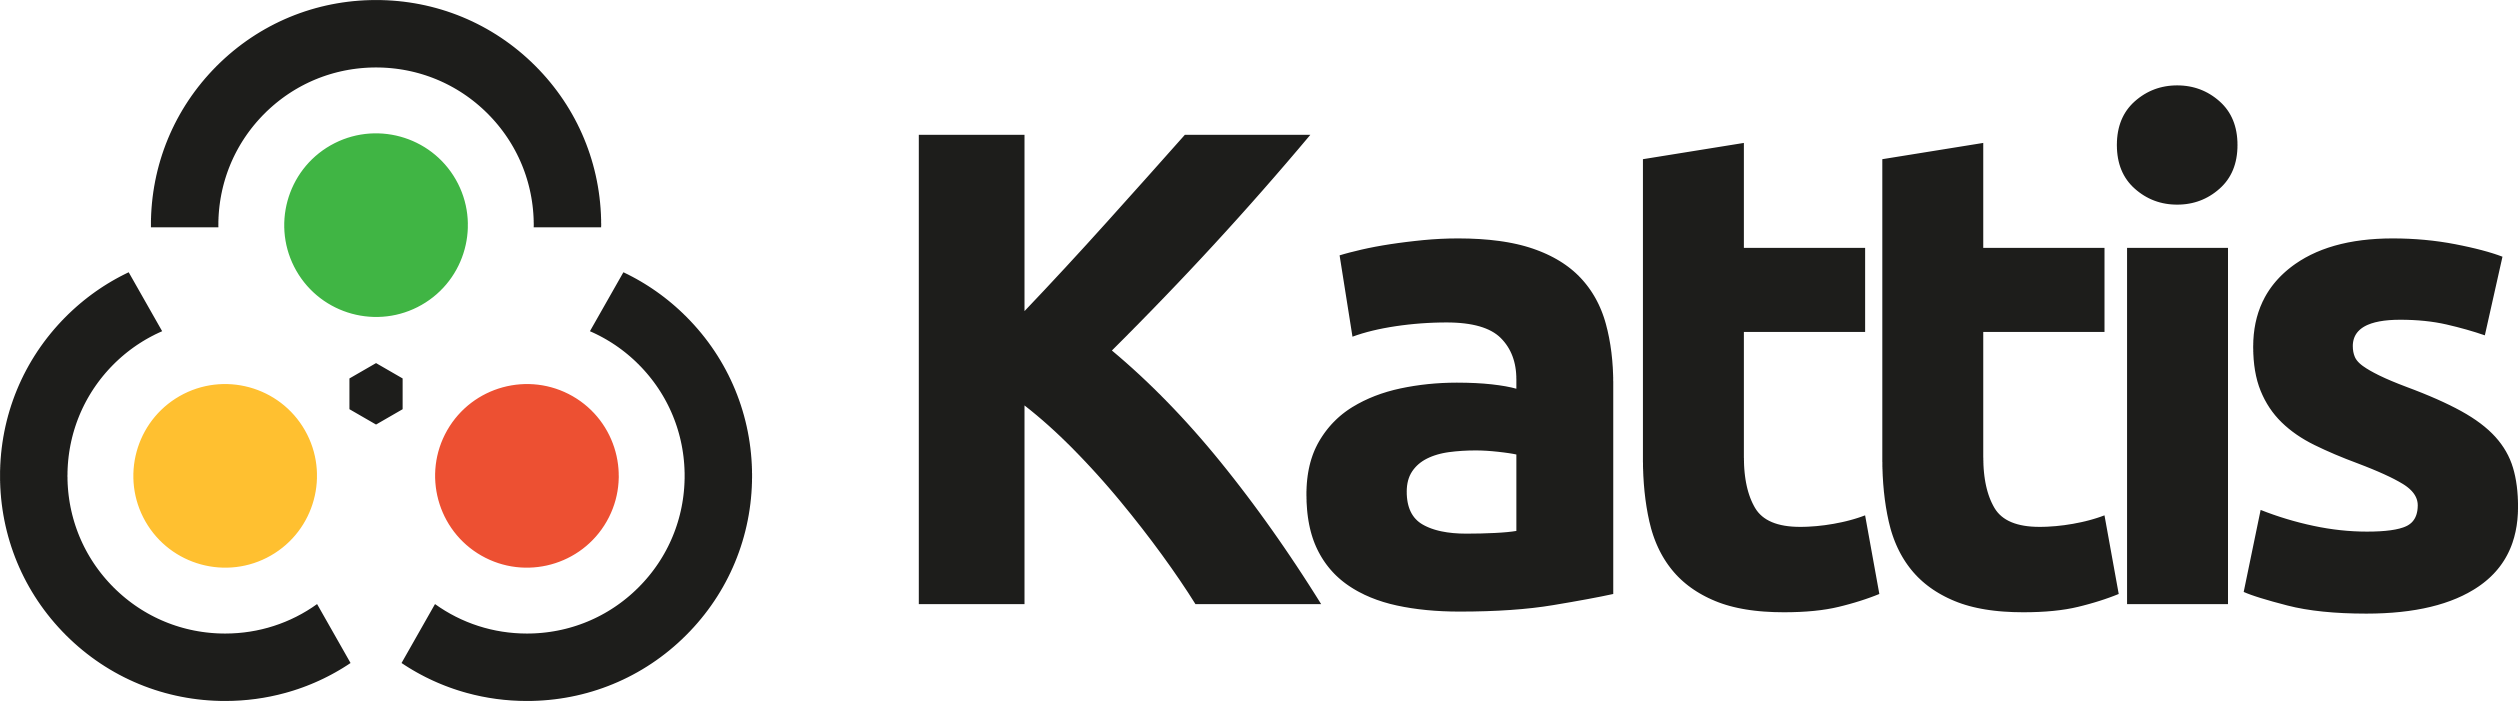
\includegraphics[height=0.6cm]{kattis}}

\begin{document}
\maketitle

\section{Divide and conquer}
\begin{frame}[plain]{Divide and conquer}
    \begin{itemize}
        \item Given an instance of the problem, the basic idea is to
        \begin{enumerate}
            \item split the problem into one or more smaller subproblems
            \item solve each of these subproblems recursively
            \item combine the solutions to the subproblems into a solution of the given problem
        \end{enumerate}

        \vspace{5pt}

        \item Some standard divide and conquer algorithms:
        \begin{itemize}
            \item Quicksort / Mergesort
            \item Karatsuba algorithm
            \item Strassen algorithm
            \item Many algorithms from computational geometry
                \begin{itemize}
                    \item Convex hull
                    \item Closest pair of points
                \end{itemize}
        \end{itemize}
    \end{itemize}
\end{frame}

\begin{frame}[plain,fragile]{Divide and conquer: Time complexity}
    \begin{minted}[fontsize=\scriptsize]{cpp}
void solve(int n) {
    if (n == 0)
        return;

    solve(n/2);
    solve(n/2);

    for (int i = 0; i < n; i++) {
        // some constant time operations
    }
}
    \end{minted}

    \begin{itemize}
        \item What is the time complexity of this divide and conquer algorithm?
        \item Usually helps to model the time complexity as a recurrence relation:
            \begin{itemize}
                \item $T(n) = 2T(n/2) + n$
            \end{itemize}
    \end{itemize}
\end{frame}

\begin{frame}[plain,fragile]{Divide and conquer: Time complexity}
    \begin{itemize}
        \item But how do we solve such recurrences?
        \item Usually simplest to use the Master theorem when applicable
            \begin{itemize}
                \item It gives a solution to a recurrence of the form $T(n) = aT(n/b) + f(n)$ in asymptotic terms
                \item All of the divide and conquer algorithms mentioned so far have a recurrence of this form
            \end{itemize}
        \vspace{10pt}
        \item The Master theorem tells us that $T(n) = 2T(n/2) + n$ has asymptotic time complexity $O(n \log n)$
        \vspace{10pt}
        \item You don't need to know the Master theorem for this course, but still recommended as it's very useful
    \end{itemize}
\end{frame}


\begin{frame}[plain,fragile]{Binary exponentiation}
    \begin{itemize}
        \item We want to calculate $x^n$, where $x,n$ are integers
        \item Assume we don't have the built-in \texttt{pow} method
        \item Naive method:
    \end{itemize}

    \begin{minted}{cpp}
int pow(int x, int n) {
    int res = 1;
    for (int i = 0; i < n; i++) {
        res = res * x;
    }

    return res;
}
    \end{minted}

    \begin{itemize}
        \item This is $O(n)$, but what if we want to support large $n$ efficiently?
    \end{itemize}
\end{frame}

\begin{frame}[plain]{Binary exponentiation}
    \begin{itemize}
        \item Let's use divide and conquer
        \vspace{10pt}
        \item Notice the three identities:

            \begin{itemize}
                \item $x^0 = 1$
                \item $x^n = x \times x^{n-1}$
                \item $x^n = x^{n/2} \times x^{n/2}$
            \end{itemize}

        \item Or in terms of our function:

            \begin{itemize}
                \item $pow(x,0) = 1$
                \item $pow(x,n) = x \times pow(x, n-1)$
                \item $pow(x,n) = pow(x, n/2) \times pow(x, n/2)$
            \end{itemize}

        \item $pow(x,n/2)$ is used twice, but we only need to compute it once:

            \begin{itemize}
                \item $pow(x,n) = pow(x, n/2)^2$
            \end{itemize}
    \end{itemize}
\end{frame}

\begin{frame}[plain,fragile]{Binary exponentiation}
    \begin{itemize}
        \item Let's try using these identities to compute the answer recursively
    \end{itemize}

    \vspace{10pt}

    \begin{minted}{cpp}
int pow(int x, int n) {
    if (n == 0) return 1;
    return x * pow(x, n - 1);
}
    \end{minted}

    \vspace{10pt}

    \begin{itemize}
        \item<2-> How efficient is this?
            \begin{itemize}
                \item $T(n) = 1 + T(n-1)$
                \item<3-> $O(n)$
                \item<4-> Still just as slow...
            \end{itemize}
    \end{itemize}

\end{frame}

\begin{frame}[plain,fragile]{Binary exponentiation}
    \begin{itemize}
        \item What about the third identity?
            \begin{itemize}
                \item $n/2$ is not an integer when $n$ is odd, so let's only use it when $n$ is even
            \end{itemize}
    \end{itemize}

    \begin{minted}{cpp}
int pow(int x, int n) {
    if (n == 0) return 1;
    if (n % 2 != 0) return x * pow(x, n - 1);
    int st = pow(x, n/2);
    return st * st;
}
    \end{minted}

    \begin{itemize}
        \item How efficient is this?
            \begin{itemize}
                \item<2-> $T(n) = 1 + T(n-1)$ if $n$ is odd
                \item<2-> $T(n) = 1 + T(n/2)$ if $n$ is even
                \item<3-> $T(n) = 1 + 1 + T((n-1)/2)$ if $n$ is odd
                \item<4-> $O(\log n)$
            \end{itemize}
    \end{itemize}
\end{frame}

\begin{frame}[plain]{Binary exponentiation}
    \begin{itemize}
        \item Notice that $x$ doesn't have to be an integer, and $\star$ doesn't have to be integer multiplication...
        \item It also works for:
            \begin{itemize}
                \item Computing $x^n$, where $x$ is a floating point number and $\star$ is floating point number multiplication
                \item Computing $A^n$, where $A$ is a matrix and $\star$ is matrix multiplication
                \item Computing $x^n \pmod{m}$, where $x$ is an integer and $\star$ is integer multiplication modulo $m$
                \item Computing $x\star x\star \cdots \star x$, where $x$ is any element and $\star$ is any associative operator
            \end{itemize}

        \item All of these can be done in $O(\log(n) \times f)$, where $f$ is the cost of doing one application of the $\star$ operator
    \end{itemize}
\end{frame}

\begin{frame}[plain]{Fibonacci words}
    \begin{itemize}
        \item Recall that the Fibonacci sequence can be defined as follows:
            \begin{itemize}
        \item $\mathrm{fib}_1 = 1$
        \item $\mathrm{fib}_2 = 1$
        \item $\mathrm{fib}_n = \mathrm{fib}_{n-2} + \mathrm{fib}_{n-1}$
            \end{itemize}
        \item We get the sequence $1, 1, 2, 3, 5, 8, 13, 21, \ldots$
        \item There are many generalizations of the Fibonacci sequence
        \item One of them is to start with other numbers, like:
            \begin{itemize}
                \item $f_1 = 5$
                \item $f_2 = 4$
                \item $f_n = f_{n-2} + f_{n-1}$
            \end{itemize}
        \item We get the sequence $5, 4, 9, 13, 22, 35, 57, \ldots$
        \item What if we start with something other than numbers?
    \end{itemize}
\end{frame}

\begin{frame}[plain]{Fibonacci words}
    \begin{itemize}
        \item Let's try starting with a pair of strings, and let $+$ denote string concatenation:
            \begin{itemize}
                \item $g_1 = A$
                \item $g_2 = B$
                \item $g_n = g_{n-2} + g_{n-1}$
            \end{itemize}
        \vspace{10pt}
        \item Now we get the sequence of strings:
        \begin{align*}
        &A, B, AB, BAB, ABBAB, BABABBAB, \\
        &ABBABBABABBAB, \\
        &BABABBABABBABBABABBAB, \ldots \\
        \end{align*}
    \end{itemize}
\end{frame}

\begin{frame}[plain]{Fibonacci words}
    \begin{itemize}
        \item How long is $g_n$?
        \begin{itemize}
            \item $\mathrm{len}(g_1) = 1$
            \item $\mathrm{len}(g_2) = 1$
            \item $\mathrm{len}(g_n) = \mathrm{len}(g_{n-2}) + \mathrm{len}(g_{n-1})$
        \end{itemize}
        \vspace{5pt}
        \item Looks familiar?
        \vspace{2pt}
        \item $\mathrm{len}(g_n) = \mathrm{fib}_{n}$
        \vspace{10pt}
        \item So the strings become very large very quickly
        \begin{itemize}
            \item $\mathrm{len}(g_{10}) = 55$
            \item $\mathrm{len}(g_{100}) = 354224848179261915075$
        \end{itemize}
    \end{itemize}
\end{frame}

\begin{frame}[plain]{Fibonacci words}
    \begin{itemize}
        \item Task: Compute the $i$th character in $g_{n}$
        \vspace{10pt}
        \item<2-> Simple to do in $O(\mathrm{len}(n))$, but that is extremely slow for large $n$
        \vspace{10pt}
        \item<3-> Can be done in $O(n)$ using divide and conquer
    \end{itemize}
\end{frame}

\begin{frame}[plain]{Mergesort}
    \begin{itemize}
        \item Input is a sequence of $n$ elements $A_1, A_2, \dotsc, A_n$.
        \item Base case when $n=1$, just return sequence
        \item Otherwise, split into two (almost) equal halves
        \item Recursively sort sequences $A_1, \dotsc A_{\lfloor\frac{n}{2}\rfloor}$ and $A_{\lfloor\frac{n}{2}\rfloor + 1}, \dotsc, A_{n}$.
        \item Create new sequence by interleaving the two, always picking the lower front value.
        \item Mergesort is an $\mathcal{O}(n \log n)$ sorting algorithm
    \end{itemize}
\end{frame}

\begin{frame}[plain]{Inversions}
    \begin{itemize}
        \item An inversion is a pair of out of order elements.
        \item Consider the permutation $6, 2, 3, 1, 5, 4$
        \item $(6, 2)$ form an inversion
        \item $(2, 5)$ do not form an inversion
        \item There are $5 + 1 + 1 + 0 + 1 + 0 = 8$ inversions in the permutation.
        \item Problem: Given permutation of size $n \leq 10^6$, compute number of inversions.
    \end{itemize}
\end{frame}

\begin{frame}[plain]{Counting inversions}
    \begin{itemize}
        \item<1-> Recall mergesort
        \item<1-> Can we modify it to count inversions?
        \item<2-> Assume it does count inversions.
        \item<2-> Mergesorting left half gives us inversions there and same for right half.
        \item<2-> Need to compute number of inversions with one element in left half and the other in right half.
        \item<3-> When picking element from right half, add number of elements remaining in left half.
        \item<3-> Since sequences are sorted, we know everything remaining in left half is larger than the picked element from right half.
    \end{itemize}
\end{frame}

\end{document}
